\section*{Exploring the Magic Formula}

In this assignment, we will move away from the Modified Fiala Tire Model that we've been using and explore the Pacejka Magic Formula tire model.  The Modified Fiala Model is a good, simple way to represent tire force generation, and we can derive it nicely from physical observations.  However, the Magic Formula is able to represent some more complex tire characteristics that often interest manufacturers and racing teams so it has evolved into the industry standard since its inception in the late 1980s.  In its more complex form, we can use it to calculate $F_x$ and $F_y$ using longitudinal slip, lateral slip, tire load, friction coefficient and wheel camber.  We've decided to introduce it here to give you exposure to what you may see in industry, not because the Fiala Model is flawed.  Quite the opposite, The Fiala Model does a very good job of representing our tire dynamics given its simplicity.

If you'd like to read more about the Magic Formula, we recommend checking out Pacejka's \textit{Tire and Vehicle Dynamics} (\url{https://www.sciencedirect.com/science/article/pii/B9780080970165000048}).  For the context of this homework, we will use a simplified Magic Formula of the form $F_{y} = f(\mu, F_z, F_x, \alpha)$ to calculate lateral force analogously to the simplified Fiala Model. 

Let's compare $F_{yf}$ and $F_{yr}$ from the two models:

\begin{center}
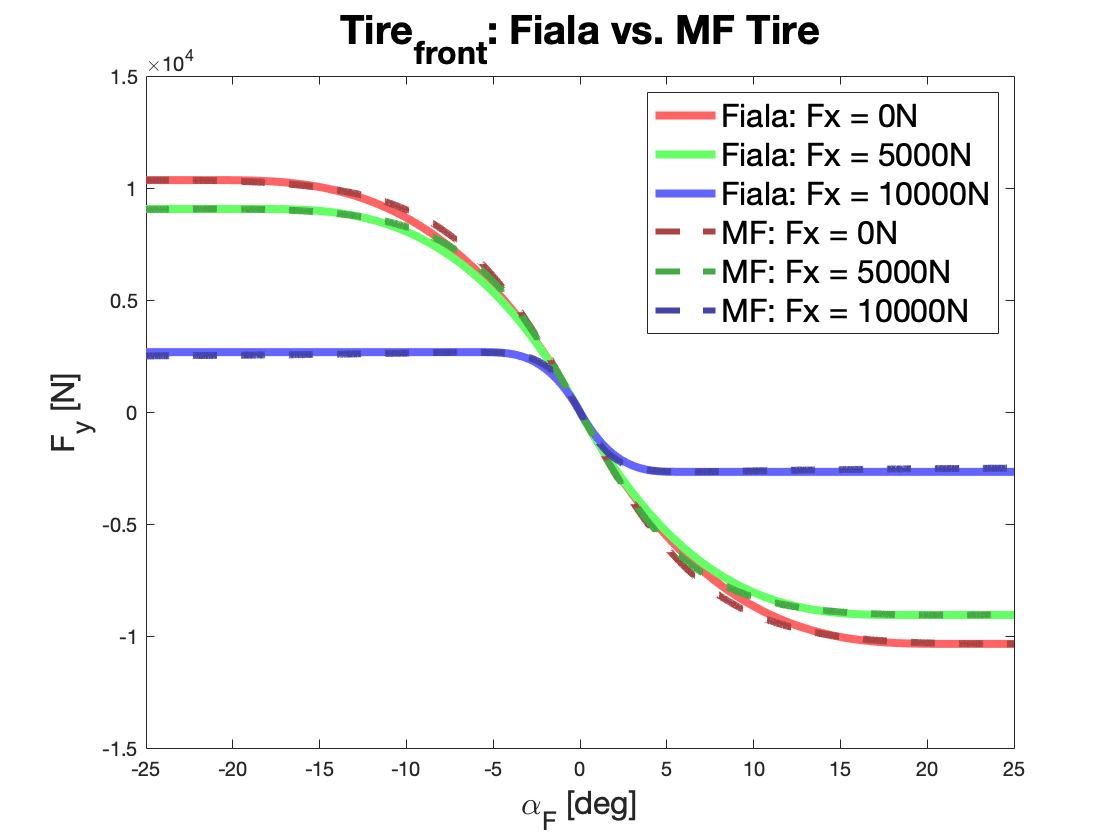
\includegraphics[width=200pt]{Body/FialaVsMF.png}
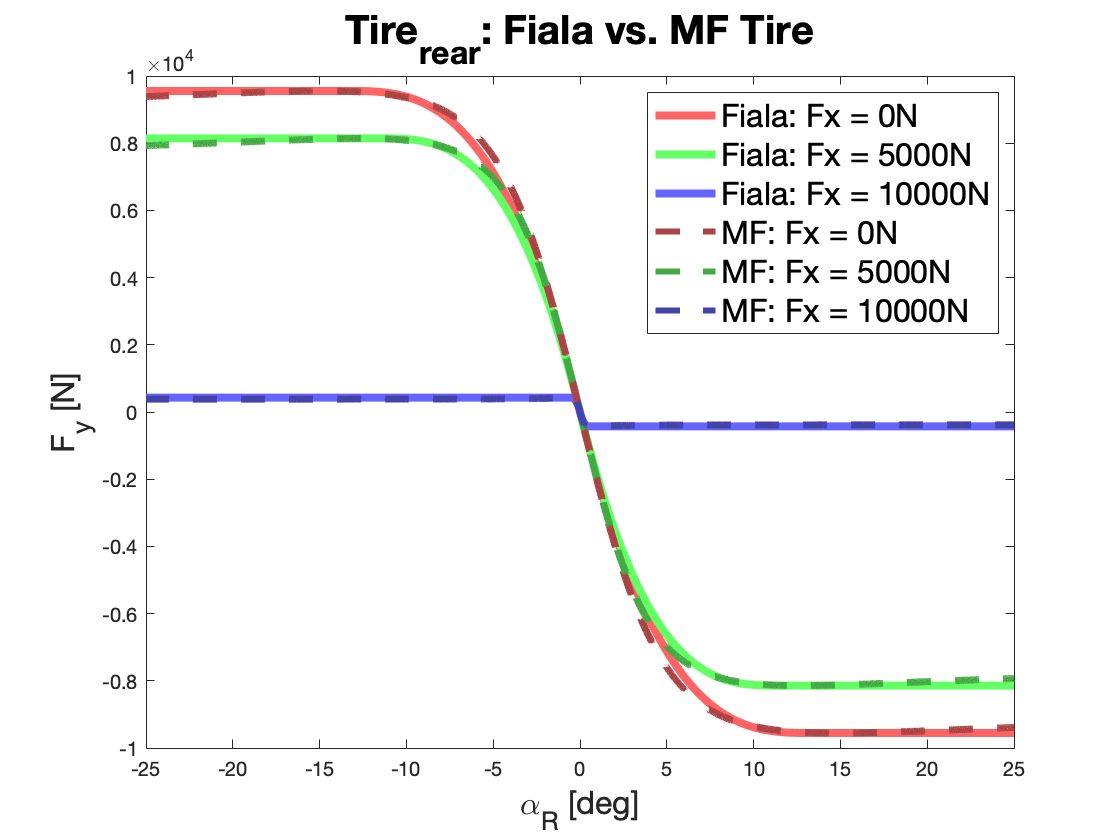
\includegraphics[width=200pt]{Body/FialaVsMF_rear.png}
\end{center}

If you're looking at the plots and saying, "these two models look pretty much the same," that is the point.  We've simply substituted one mathematical representation for our tires for another, both tuned for the same set of tires. We can notice some difference between the curves in the slip range between the linear and saturated regions, and that is where these models tend to differ slightly with the Magic Formula more closely matching recorded data. 

The Teaching Team has taken care of implementation of the Magic Formula in \verb!MF_tire.m!.  Nonetheless, we do recommend checking out the magic behind the Magic Formula in some of Pacejka's papers.